\section{Experimental Setup}
To evaluate the effectiveness of our symmetry elimination technique we performed
a comparative analysis using A* on a set of 120 grid maps taken from BioWare's 
popular roleplaying game \emph{Baldur's Gate 2}. 
Figure \ref{fig-bgmap} shows a typical example.
These maps range in size from 50x50 to 320x320 and are a commonly used benchmark 
that often appears in the literature 
\cite{botea04,bjornsson05,bjornsson06,sturtevant05,harabor08}.
%We believe these maps are sufficiently representative of scenarios typical to modern video games. 
 \begin{figure}[b]
        \begin{center}
                        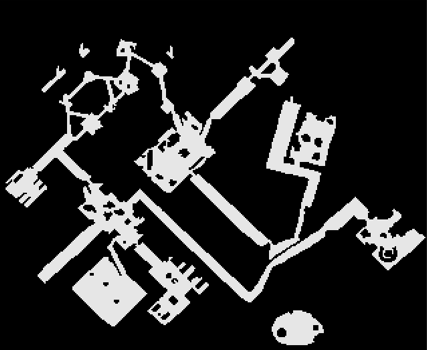
\includegraphics[width=0.8\columnwidth, trim = 10mm 10mm 10mm 0mm]{diagrams/bgmap.png}
        \end{center}
        \caption{An example map from BioWare's \emph{Baldur's Gate 2}}
        \label{fig-bgmap}
 \end{figure}
\par
We also evaluate A* on the demo map from Figure \ref{fig-contrast},
 which is distributed with the University of Alberta's freely available pathfinding library 
Hierarchical Open Graph\footnote{\url{www.cs.ualberta.ca/~nathanst/hog.html}} (or HOG).
This map has similar characteristics to maps from the Baldur's Gate set (being comprised of rooms
connected by corridors) but unlike those maps it is not rotated by 45 degrees. 
We use six variants of this map which we designate \emph{R0, R10, R20, R30, R40, R50}.
In each case the numeric constant refers to the probability that each traversable tile 
in the original map will be be flipped to become an obstacle.
We added these extra maps in order to measure the worst case performance of A* which we expect will occur in 
environments that are densely packed with obstacles.
\par
For each map we generated 100 experiments by randomly creating valid problems between arbitrarily chosen 
pairs of start and goal locations.
Each algorithm solved every problem once making for a total of 25200 (126 $\times$ 200) distinct experiments.
All experiments were conducted on a 1.83GHz Intel Core 2 Duo processor with 1GB RAM running OSX 10.5.4.
A* is implemented using HOG.
